\documentclass[12pt,oneside]{article}
\usepackage[utf8]{inputenc}
\usepackage{float}
\usepackage[bottom]{footmisc}
\usepackage{bookmark}
\usepackage{microtype}
\usepackage{amsmath}
\usepackage{multicol}
\usepackage{mdframed}
\usepackage{setspace}
\usepackage{pgfplots}
\usepackage{graphicx}
\usepackage{fancyvrb}
\usepackage[absolute]{textpos}\TPGrid{16}{16}
\usepackage{tikz}
  \usetikzlibrary{shapes}
  \usetikzlibrary{arrows.meta}
  \usetikzlibrary{arrows}
  \usetikzlibrary{shadows}
  \usetikzlibrary{trees}
  \usetikzlibrary{fit}
  \usetikzlibrary{calc}
  \usetikzlibrary{positioning}
  \usetikzlibrary{decorations.pathmorphing}
\usepackage{./tikz-uml}
\usepackage{everypage}
  \AddEverypageHook{
    \begin{textblock}{0.5}[0,0](0,0)
      \tikz \node[fill=mypink,minimum width=0.5\TPHorizModule,minimum height=16\TPVertModule] {};
    \end{textblock}
    \begin{textblock}{0.125}[0,0](0.5,0)
      \tikz \node[fill=myblack,inner sep=0, minimum width=0.125\TPHorizModule,minimum height=16\TPVertModule] {};
    \end{textblock}
  }
\usepackage{xcolor}
  \definecolor{firebrick}{HTML}{B22222}
  \definecolor{myred}{HTML}{CF0A2C}
  \definecolor{mypink}{HTML}{560CCE}
  \definecolor{myblack}{HTML}{232527}
\newcommand\dd[1]{\colorbox{gray!30}{\texttt{#1}}}
\usepackage{hyperref}
  \hypersetup{colorlinks=true,allcolors=blue!40!black}
\setlength{\topskip}{6pt}
\setlength{\parindent}{0pt} % indent first line
\setlength{\parskip}{6pt} % before par
% \let\oldsection\section\renewcommand\section{\newpage\oldsection}
\date{\small\today}
\title{%
  MkDrop: Tokens Flow Management\\
  \colorbox{mypink}{\small\sffamily\color{white}{White Paper}}}
\usepackage[style=authoryear,sorting=nyt,backend=biber,
  hyperref=true,abbreviate=true,
  maxcitenames=1,maxbibnames=1]{biblatex}
  \renewbibmacro{in:}{}
  \addbibresource{books.bib}
\tikzset{node distance=1.6cm, auto, every text node part/.style={align=center, font={\sffamily\small}}}
\tikzstyle{block} = [draw=myblack, fill=white, inner sep=0.3cm, outer sep=0.1cm, thick]
\tikzstyle{ln} = [draw, ->, very thick, arrows={-triangle 90}, every text node part/.append style={font={\sffamily\scriptsize}}]
\author{Bohdan Snisar \and Yurii Chudinov} % Add authors here
\begin{document}
\raggedbottom

\maketitle
\begin{abstract}
  In the rapidly evolving landscape of cryptocurrency, the distribution of tokens, 
  particularly through airdrops, plays a pivotal role in project promotion 
  and community engagement. However, the current methods for token distribution 
  are fraught with challenges like high transaction costs, security risks, and 
  inefficient processes. This white paper proposes a novel platform designed to 
  streamline and secure the process of token distribution while maintaining the 
  anonymity characteristic of the crypto world.
\end{abstract}

% \onehalfspace

\section{Introduction}
The realm of cryptocurrency has been rapidly expanding with new projects.
A critical element for the success of these projects is the effective distribution of tokens, often through
airdrops, to build and maintain community engagement. This white paper introduces 
a new platform that automates token distribution, enhances security, and 
fosters authentic community growth.

Token distribution is an integral part of cryptocurrency projects, providing a mechanism 
for allocating digital assets to various stakeholders, including investors, team members, and users.
 Over the years, the methods and models of 
token distribution has evolved, reflecting the changing landscape of the 
cryptocurrency industry and its growing complexity. 

\begin{description}
  \item[Initial Coin Offerings (ICOs)]
  Starting around 2013, ICOs emerged as a popular method for crypto projects to raise funds.
  Investors would contribute, typically in Bitcoin, to early developers in exchange for 
  tokens at network launch. This method saw massive popularity, with projects 
  like Ethereum raising significant funds through ICOs.

  \item[Venture Capital Investment]
  Another traditional method involves venture capitalist firms investing 
  in crypto startups by purchasing their tokens. This model differs from 
  traditional venture capital as it focuses on token acquisition rather than company equity.

  \item[Airdrops]
  Airdrops have been used as a marketing strategy to distribute a small number of tokens 
  to users' digital wallets. This approach helps in creating awareness about the project 
  and fostering a network effect.

  \item[Lockdrops]
  Lockdrops are a unique distribution process where users lock up their existing 
  tokens for a certain period before the launch of a new cryptocurrency project. 
  This model relies on the commitment of participants to the success of the new project.

  \item[Public Sales]
  This includes methods like Initial Exchange Offerings (IEOs) and Initial DEX Offerings (IDOs), 
  where tokens are introduced to the market via exchanges, offering a decentralized approach 
  to token distribution.
\end{description}


\section{Challanges}

In the dynamic world of cryptocurrency projects, the deployment of token vesting schedules 
is a critical aspect that demands careful consideration. Vesting schedules, once encoded 
into smart contracts, become immutable. While this immutability serves the purpose 
of ensuring transparency and trust, it also introduces a layer of rigidity that can 
be challenging, particularly for projects whose roadmaps are still evolving.


\begin{description}
  \item[Inflexibility to Project Evolution]
  In the early, often changing phases of cryptocurrency projects, the unchangeable nature
   of vesting schedules in smart contracts can 
  lead to a misalignment between evolving project needs and set token distribution plans.

  \item[Impact on Stakeholder Trust and Project Perception]
  Stakeholders' trust can be significantly impacted if the project's direction shifts 
  substantially after the airdrop or initial distribution. Immutable schedules can
  leave stakeholders feeling disadvantaged, potentially affecting their ongoing
  support and trust in the project.

  \item[Operational and Strategic Constraints]
  Fixed vesting schedules can limit the project team's ability to make 
  strategic adjustments. This includes altering the project scope, 
  extending development timelines or pivoting the project strategy 
  in response to market feedback, technological advances, or 
  changes in the project's ecosystem.
\end{description}


\section{Solution}

The "Provisional Token Allocation" approach involves initially reserving tokens 
for users without directly allocating them to their wallets. 

Instead, users are provided with placeholders or "slots" representing their entitlement to tokens. 
These slots remain provisional until certain criteria or milestones are met, at which point 
the tokens are materialized or converted into immutable tokens. 

The criteria for materialization 
can vary, including project milestones, market conditions, or predefined time-based factors. 
This approach offers flexibility in the timing of token distribution.

Keynotes from the process flow:
\begin{enumerate}
  \item \textbf{Token Allocation by Company:} The starting point where the company determines and allocates tokens.
  \item \textbf{Wallet Verification:} Users undergo a verification process to ensure uniqueness. 
  Uniqueness must satisfy only proof of \textbf{one user} == \textbf{one wallet} and not aim to reveal users' identities. 
  \item \textbf{Provision:} Users claim their tokens, resulting in the assignment of 'provisional' tokens. Such tokens signifying a placeholder for future tokens and just exists on user wallets as a slots.
  \item \textbf{Materialization:} The provisional tokens are materialized into actual tokens. Materialization means a linkage them from a placeholder contract 
  to a real smart contract, embedding business logic such as vesting and other features. 
  By it's nature this process follow the intuition of \href{https://en.wikipedia.org/wiki/Late_binding} that is well known concept in software development. 
  \item \textbf{Distribution:} The actual tokens are then distributed to the end users.
\end{enumerate}

\begin{figure}[H]
  \centering
  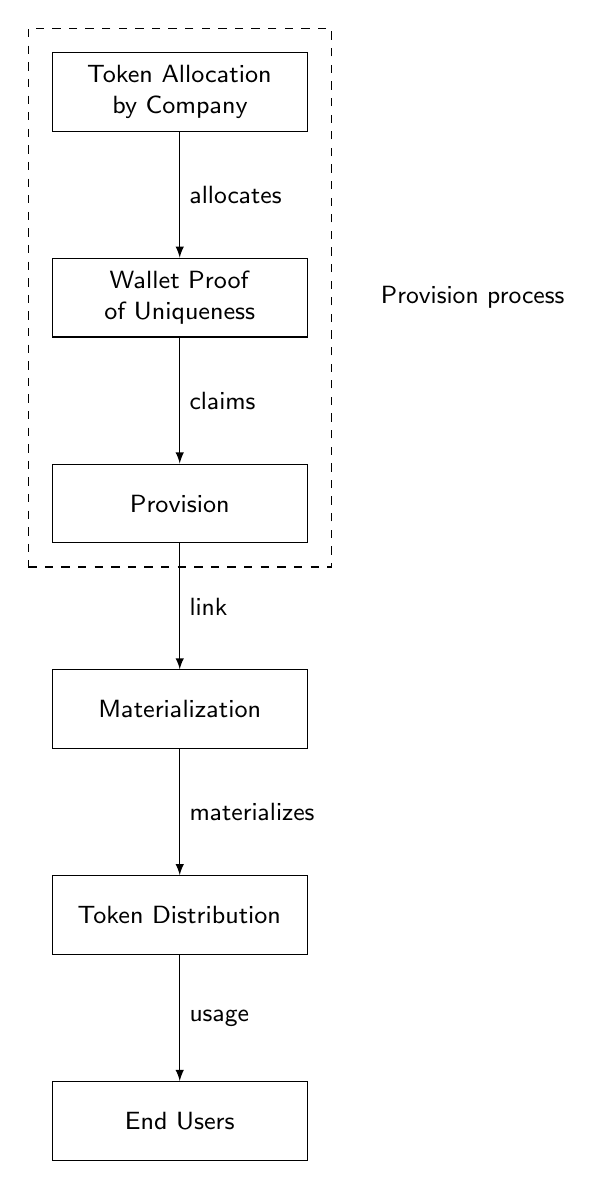
\begin{tikzpicture}[block/.style={rectangle, draw, text width=3cm, align=center, minimum height=1cm}, >=latex]
    % Nodes
    \node[block] (alloc) {Token Allocation by Company};
    \node[block, below=of alloc] (verify) {Wallet Proof of Uniqueness};
    \node[block, below=of verify] (provision) {Provision};

    % Dashed container with description
    \node[fit=(alloc)(verify)(provision), dashed, draw, inner sep=0.3cm] (container) {};
    \node[right=0.5cm of container] {Provision process}; % Label on the right

    \node[block, below=of provision] (materialize) {Materialization};
    \node[block, below=of materialize] (distribution) {Token Distribution};
    \node[block, below=of distribution] (users) {End Users};
  
    % Paths
    \draw[->] (alloc) -- node[right] {allocates} (verify);
    \draw[->] (verify) -- node[right] {claims} (provision);
    \draw[->] (provision) -- node[right] {link} (materialize);
    \draw[->] (materialize) -- node[right] {materializes} (distribution);
    \draw[->] (distribution) -- node[right] {usage} (users);
  \end{tikzpicture}
  \caption{Token Allocation Process with Provisional Tokens.}
  \label{fig:token_allocation_prov}
\end{figure}


\section{Requirements}
\label{sec:requirements}

Token desctribution at this moment solvels in a different ways: .......
Even though each of them partially solvesl described issues, neither one is perfect.

\subsection{Features}
\label{sec:features}

There are many important qualities and features cryptocomunity expects a airdrop platform to have,
in order to be useful the web3 ecosystem. The most critical \href{https://en.wikipedia.org/wiki/Functional_requirement}{functional requirements}
are:

\begin{description}
  \item[XXXXXX]
  To be written...

  \item[XXXXXX]
  To be written...

  \item[XXXXXX]
  To be written...

  \item[XXXXXX]
  To be written...

  \item[XXXXXX]
  To be written...
\end{description}

\subsection{Non-functional Requirements}
\label{sec:nfr}

The most important \href{https://en.wikipedia.org/wiki/Non-functional_requirement}{non-functional requirements} are:

\begin{description}
  \item[Security]
  This is paramount in blockchain systems to protect against fraud, hacks,
   and unauthorized access. Security measures could include multi-factor authentication, 
  encryption, secure smart contract coding practices, and regular security audits

  \item[Scalability]
  The system should be able to handle increasing workloads and 
  accommodate growth in user numbers and transaction volumes. Potential rarer but peak volumes during short timeframe.  
  This might involve off-chain processing claims, optimizing smart contract efficiency,
  considering layer 2 scaling solutions, or implementing sharding techniques

  \item[Cost Efficiency]
  Managing transaction costs, especially on networks with high gas fees, 
  is crucial for both the users and the company. 
  Optimizing smart contract execution and considering gas-efficient 
  algorithms are important in this regard.

  \item[XXX]
  to be written...

\end{description}

There are many other essential features required, including
..... and so on.

\section{Architecture}

Architecure is consisted of 4 essential parts:

% \begin{enumerate}
% 	\item HTTP layer
%         \item Authorization and authentication layer
% 	\item Repositories
% 	\item Storage
% \end{enumerate}
% \begin{tikzpicture}
%   \node[block] (repo-2) {Repo};
%   \node[block, left=of repo-2] (repo-1) {Repo};
%   \node[block, right=of repo-2] (repo-3) {Repo};
%   \node[fit=(repo-1)(repo-2)(repo-3), draw, dashed, inner sep=1cm, label={[right=10cm, below=0.1cm]1cm:Repositories}] (repos) {};
%   \node[block, above=of repos, minimum width=7cm] (auth) {authentication};
%   \node[block, above=of auth, minimum width=7cm] (http) {HTTP layer, routing and dispatching};
%   \node[block, below=of repo-1] (storage-1) {Storage};
%   \node[block, below=of repo-2] (storage-2) {Storage};
%   \node[block, below=of repo-3] (storage-3) {Storage};
%   \path[ln] (repo-1) -- (storage-1);
%   \path[ln] (repo-2) -- (storage-2);
%   \path[ln] (repo-3) -- (storage-3);
%   \path[ln] (http) -- (auth);
%   \path[ln] (auth) edge node {routes} (repos);
%   \draw (repos.north) -- (repo-1.north);
%   \draw (repos.north) -- (repo-2.north);
%   \draw (repos.north) -- (repo-3.north);
% \end{tikzpicture}


\subsection{Extensions}
to be written...

\section{Conclusion}
\label{sec:conclusion}

To be written...

\printbibliography%
\end{document}
